\newpage
\subsubsection{ESP}
\label{subsubsec:ESP}

Für die Implementierung des WiFi's wird das ESP32 verwendet. Die Hauptfunktion im Schema ist die Kommunikation mit dem Mikrocontroller über die zweite serielle Schnittstelle. Die Ansteuerung zum Schreiben des Programmspeichers muss so gestaltet werden, dass der Boot-Modus automatisch gestartet werden kann, wenn ein Code hochgeladen werden soll. Dies hat eine zusätzliche Schaltung zur Folge. 

\paragraph{Schema (WiFi-Modul)}\mbox{}

In Abbildung \ref{fig:Schema_ESP32} wird das Schema rund um das ESP32 an sich gezeigt. Es beinhaltet Stütz- und Filterkondensatoren sowie einige Pull-up- und Pull-down-Widerstände, welche verwendet werden, um einen definierten Grundzustand beim Booten des ESP32-Moduls zu erreichen (Strapping-Pins). Weiter gibt es einen Kondensator, welcher dazu da ist, bei gewünschter Zeit in den Boot-Modus zu gelangen. 

\begin{figure}[h!]
	\centering
	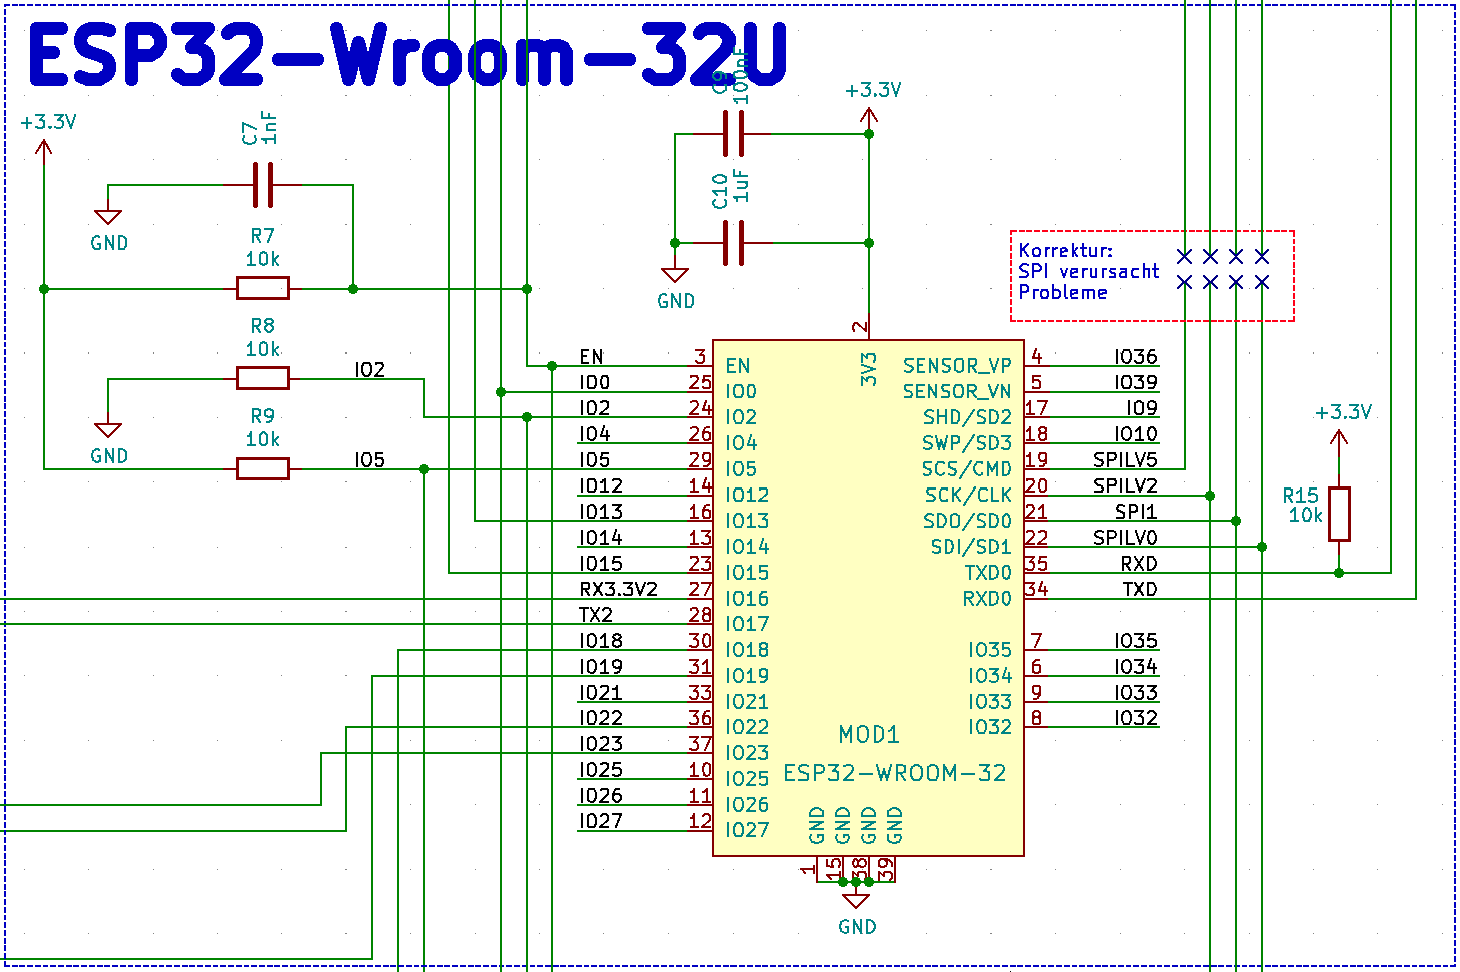
\includegraphics[width=0.5\textwidth]{graphics/Schema_ESP32}
	\caption{Schema ESP32-Wroom-32U.}
	\label{fig:Schema_ESP32}
\end{figure}

\paragraph{Funktionsbeschrieb (WiFi-Modul)}\mbox{}

Das ESP32 ist mit MOD1 beschriftet, es übernimmt die in Kapitel \ref{subsec:Wirelessmodul} beschriebenen Funktionen. Die Kondensatoren C9 und C10 dienen zu Stütz- und Filterzwecken am Spannungseingang. Der Widerstand R7 ist ein Pull-Up für Chip-Enable. Die Widerstände R8, R9, R10 und R11 dienen dazu, die Eingänge der Strapping-Pins anzusteuern. Über diese werden der Boot-Modus, die Versorgungsspannung von VDD\_SDIO\footnote{Secure Digital Input Output}-Slave (Erweiterung der SD-Spezifikationen) und andere Initialisierungseinstellungen konfiguriert. Details zu den Konfigurationen sind in Tabelle \ref{tab:Strapping_pins} aufgelistet\footnote{https://www.espressif.com/sites/default/files/documentation/esp32\_datasheet\_en.pdf S.13}. Mit dem Kondensator C7 wird sichergestellt, dass nach einem Reset der Bootmodus gestartet werden kann. Über den EN-Pin wird das Modul ein- und ausgeschaltet (acitve high).

\paragraph{Schema (Automatische Boot-Logik)}\mbox{}

In Abbildung \ref{fig:Schema_ESP32_Flashbuttons} wird die Schaltung gezeigt, welche verwendet wird, das ESP32-Modul in den gewünschten Boot-Zustand zu bringen. Für die Beschaltung der automatischen Boot-Logik benötigt es eine XNOR-Schaltung mit DTR und RTS als Input und EN und IO0 als Outputs. Die Buttons können bei Bedarf verwendet werden, sind für den automatischen Boot-Modus jedoch nicht nötig.

\begin{figure}[h!]
	\centering
	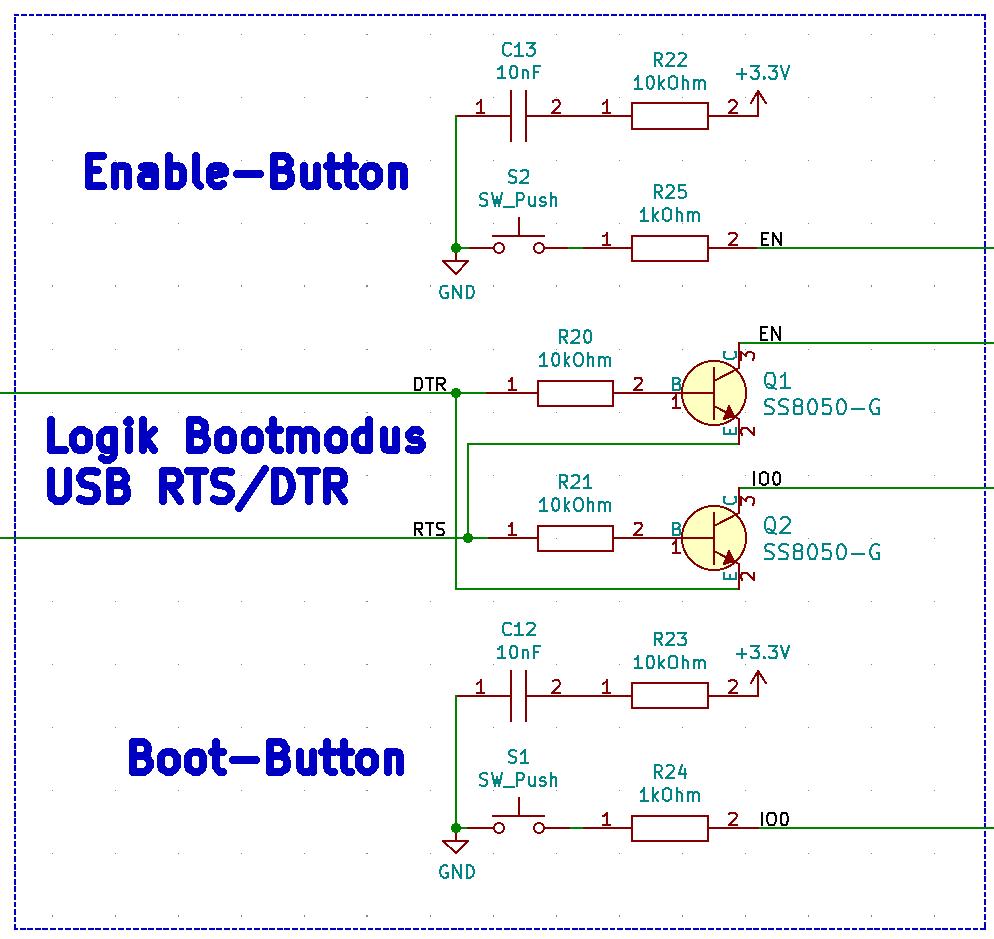
\includegraphics[width=0.5\textwidth]{graphics/Schema_ESP32_Flashbuttons}
	\caption{Schema ESP32-Wroom-32U.}
	\label{fig:Schema_ESP32_Flashbuttons}
\end{figure}

\paragraph{Funtionsbeschrieb der Schaltung (Automatische Bootlogik)}\mbox{}

Mit der Schaltung kann das ESP32-Modul mit einer bestimmten Signalabfolge an den Leitungen DTR und RTS in einen Bestimmten Boot-Modus gesetzt werden:

Wenn DTR LOW ist und RTS von HIGH nach LOW wechselt, wird der Run-Modus gestartet.\\
Wenn RTS HIGH ist und DTR von LOW nach HIGH wechselt, wird der automatische Bootloader gestartet.

\todo{Referenz einfügen: http://loboris.eu/ESP32/ESP32\_AutoReset.jpg}



\newpage



\newpage

\begin{table}[h!]
\newcolumntype{Y}{>{\centering\arraybackslash}X}
\center
\begin{tabularx}{\textwidth}{|c|c|c|Y|Y|Y|Y|}
\hline
\multicolumn{7}{|c|}{\textbf{Ausgangsspannung internen Spannungsregler (VDD\_SDIO)}}\\
\hline
RS232 & ESP & default & \multicolumn{2}{|c|}{\textbf{3.3V}} & \multicolumn{2}{|c|}{\textbf{1.8V}}\\
\hline
\sout{RTS} & \sout{IO12} & Pull-down & \multicolumn{2}{|c|}{\sout{\textcolor{red}{0}}\footnotemark} & \multicolumn{2}{|c|}{\sout{1}}\\
\hline
\multicolumn{7}{|c|}{\textbf{Boot-Modus}}\\
\hline
RS232 & ESP & default & \multicolumn{2}{|c|}{\textbf{SPI-flash Boot}} & \multicolumn{2}{|c|}{\textbf{Download Boot}}\\
\hline
DTR & IO0 & Pull-up & \multicolumn{2}{|c|}{1} & \multicolumn{2}{|c|}{0}\\
\hline
- & IO2 & Pull-down & \multicolumn{2}{|c|}{Egal} & \multicolumn{2}{|c|}{0}\\
\hline
\multicolumn{7}{|c|}{\textbf{Debugging Log Print über U0TXD während Booten}}\\
\hline
RS232 & ESP & default & \multicolumn{2}{|c|}{\textbf{U0TXD Active}} & \multicolumn{2}{|c|}{\textbf{U0TXD Silent}}\\
\hline
RTS & IO12 & Pull-down & \multicolumn{2}{|c|}{\textcolor{red}{1}} & \multicolumn{2}{|c|}{0}\\
\hline
\multicolumn{7}{|c|}{\textbf{Timing\footnotemark des SDIO}}\\
\hline
RS232 & ESP & default & FF Sampling \newline FF Output & FF Sampling \newline SF Output & SF Sampling \newline FF Output & SF Sampling \newline SF Output \\
\hline
CTS & IO15 & Pull-up & 0 & 0 & 1 & 1 \\
\hline
- & GPIO5 & Pull-up & 0 & 1 & 0 & 1 \\
\hline
\end{tabularx}

\caption{Tabelle Pinkonfiguration für Strapping-Pins.}
\label{tab:Strapping_pins}
\end{table}
\footnotetext[5]{Da das ESP32-WROOM-32U einen 3.3V SPI flash integriert hat, kann der MTDI nicht auf 1 gesetzt werden, wenn die Module aufgestartet sind.}
\footnotetext{FF = Fallende Flanke, SF = Steigende Flanke}


\textbf{Spannung des internen Spannungsgeglers (VDD\_SDIO)}

Das ESP32 hat einen eingebauten host controller für SD/SDIO/MMC-Speichergeräte. Dieser kann mit 3.3V (IO12 = 0) oder 1.8V (IO12 = 1) betrieben werden. Wird der Pin auf 1 gesetzt, könnte ein Brown-out der IO-Versorgungspannung VCC\_IO ausgelöst werden.

\textbf{Booting Mode}
Der Pin IO0 gibt vor, ob das ESP32 vom internen SPI-flash bootet (IO0 = 1) oder ob neuer Code in den flash Speicher geschrieben wird (IO0 = 0). Soll das ESP vom Flash-Speicher booten, so hat der Pin IO2 kein Einfluss, um jedoch den Code speichern zu können, muss der Pin auf 0 sein.

\textbf{De-/Aktivieren vom Debug-Log über U0TXD während dem Bootvorgang}

Über den Pin IO12 kann konfiguriert werden, ob während dem Booten ein Debug-Log über die Serielleschnittstelle gesendet wird (IO12 = 1) oder nicht (IO12 = 0). 

\textbf{Timing der Kommunikation mit dem SDIO Slave}:

Über die Pins IO15 und IO5 kann das Übertragungsprotokoll des SDIO-Slaves festgelegt werden. Dabei kommt es darauf an, ob das Sampling auf eine fallende Flanke (IO15 = 0) oder steigende Flanke (IO15 = 1) geschehen soll, und ob der Output auf eine fallende Flanke (IO5 = 0) oder steigende Flanke (IO5 = 1) geschehen soll.

\newpage